\begin{GreyBox}
    \vskip-1cm
    \begin{block}{\GHead{Application}}

        \begin{columns}[c]
            \column{0.3\textwidth}
                \begin{flushleft}
                    \hskip5cm\textcolor{TitleBlue}{\textbf{OH Reactivity}}
                    \vskip3cm
                    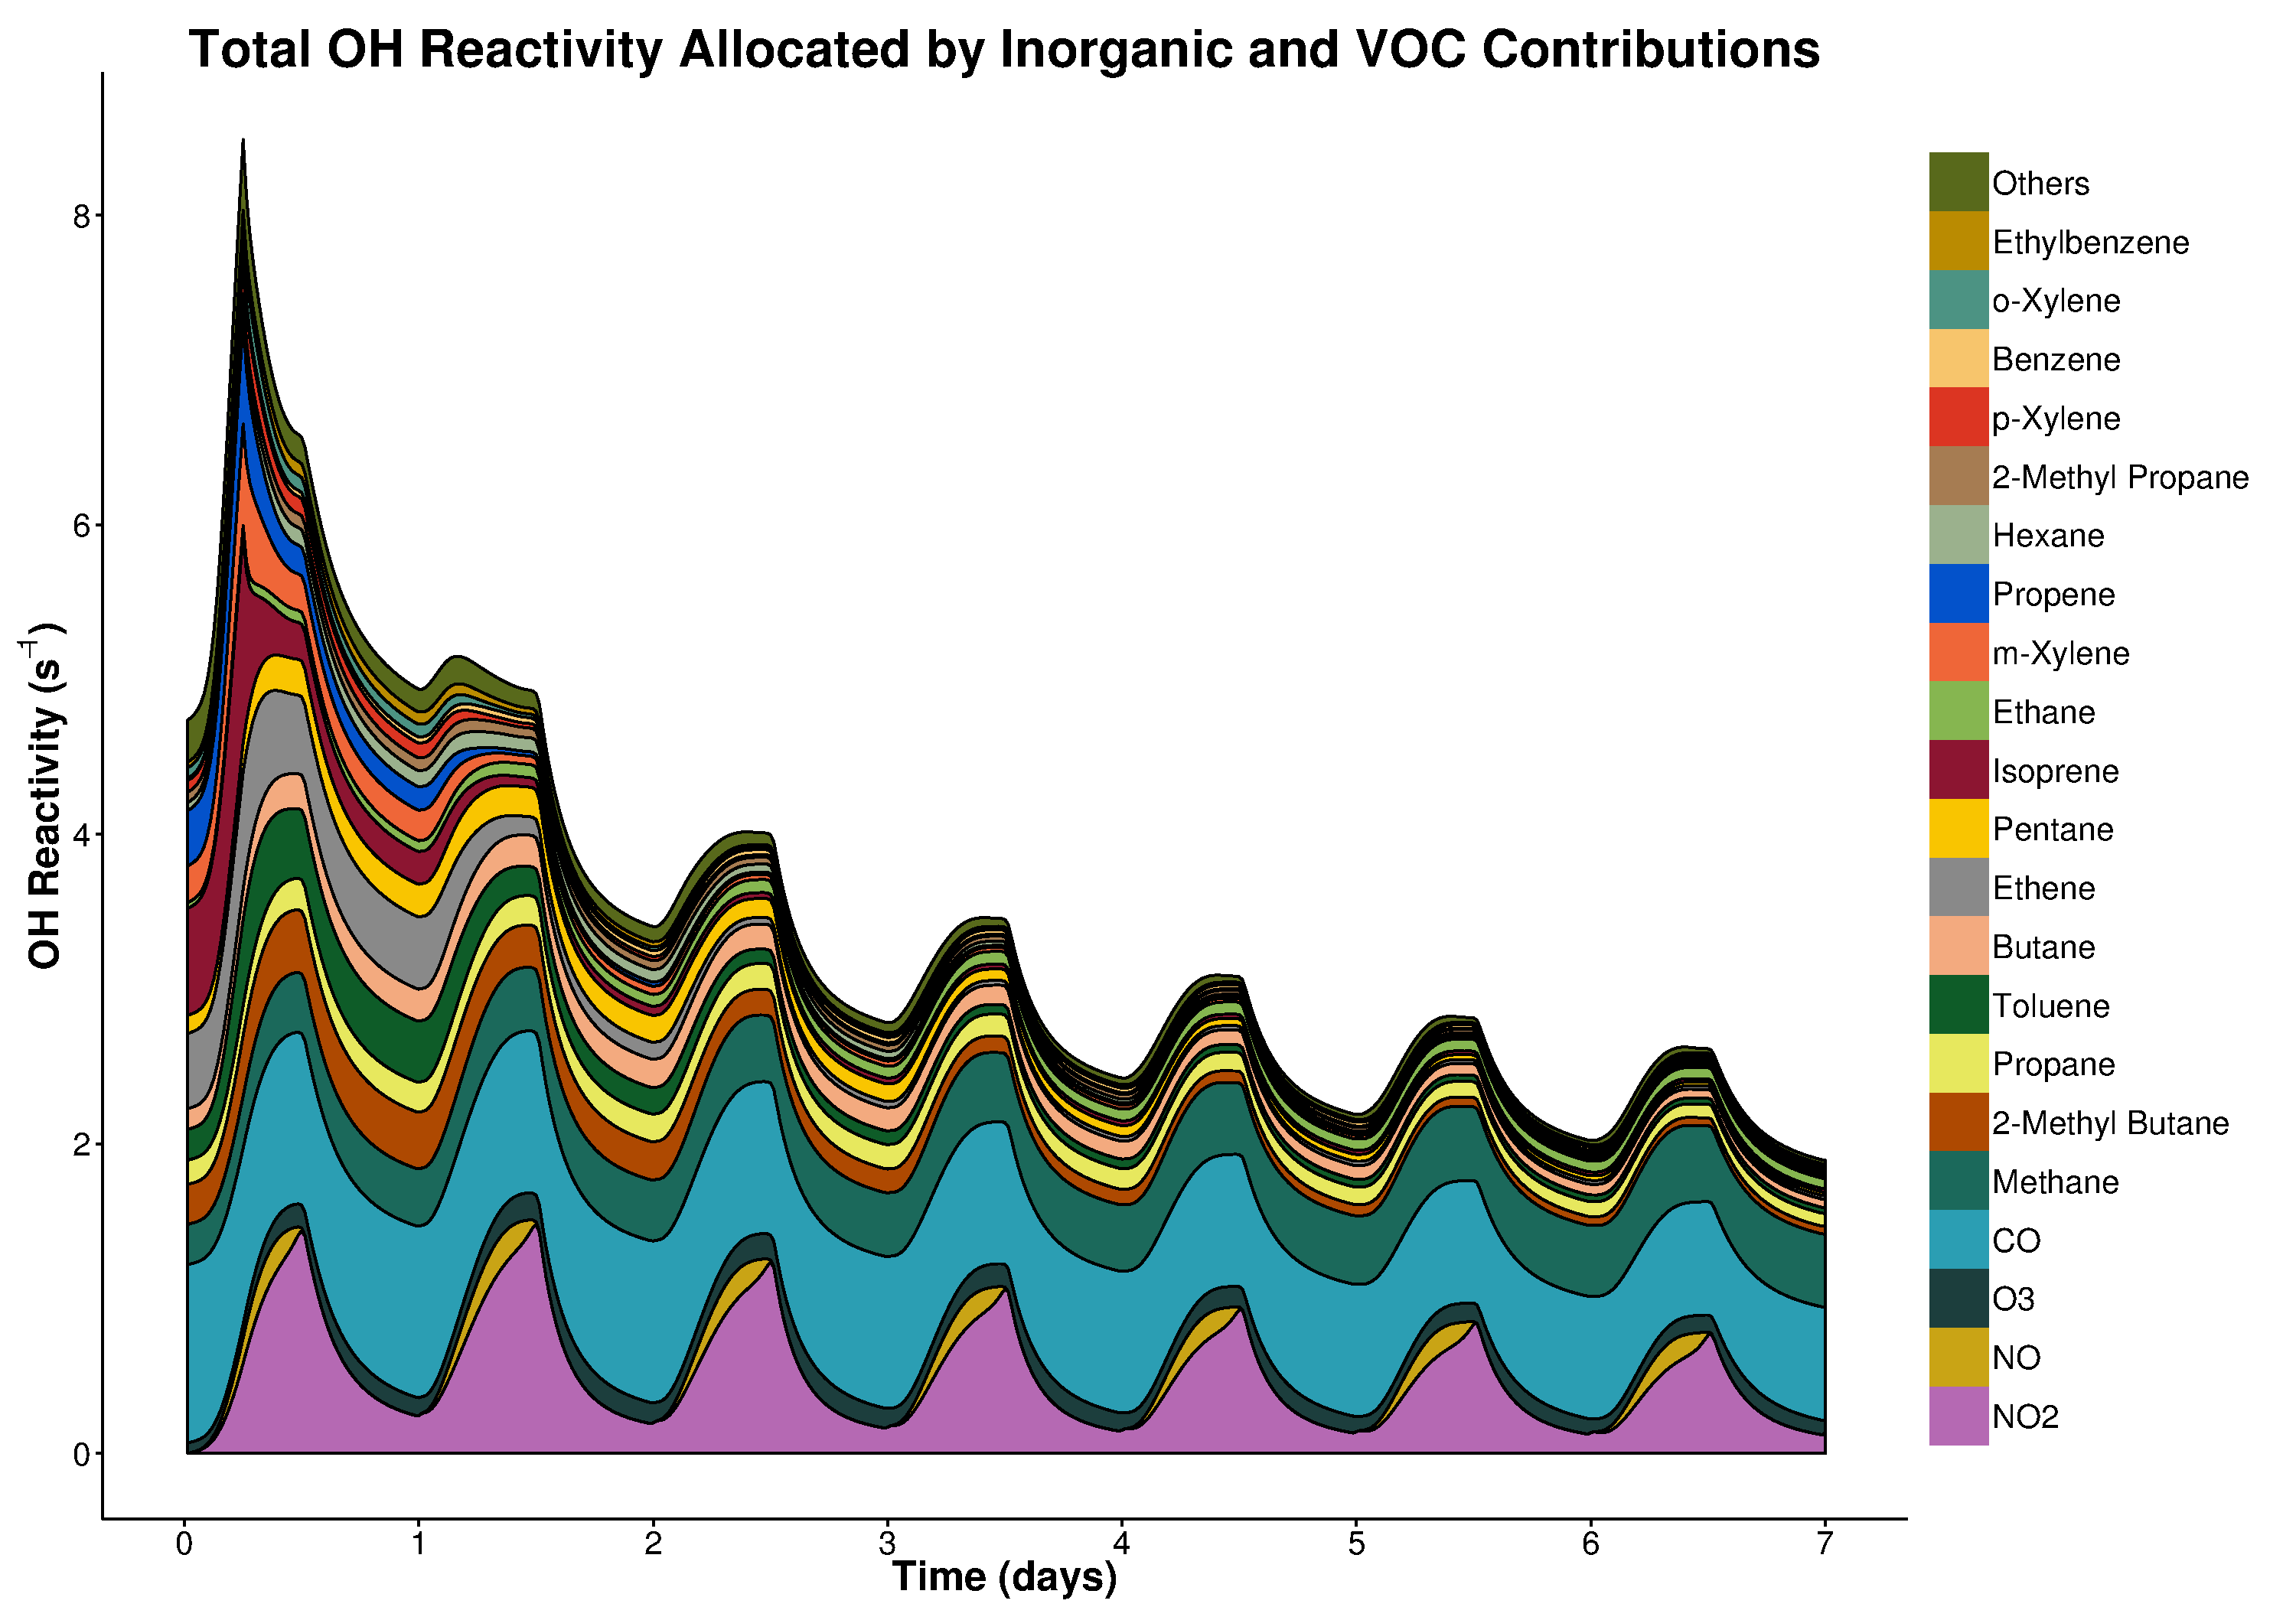
\includegraphics[scale=0.43]{img/OH_reactivity_allocation_time_series}
                    \vskip6cm
                    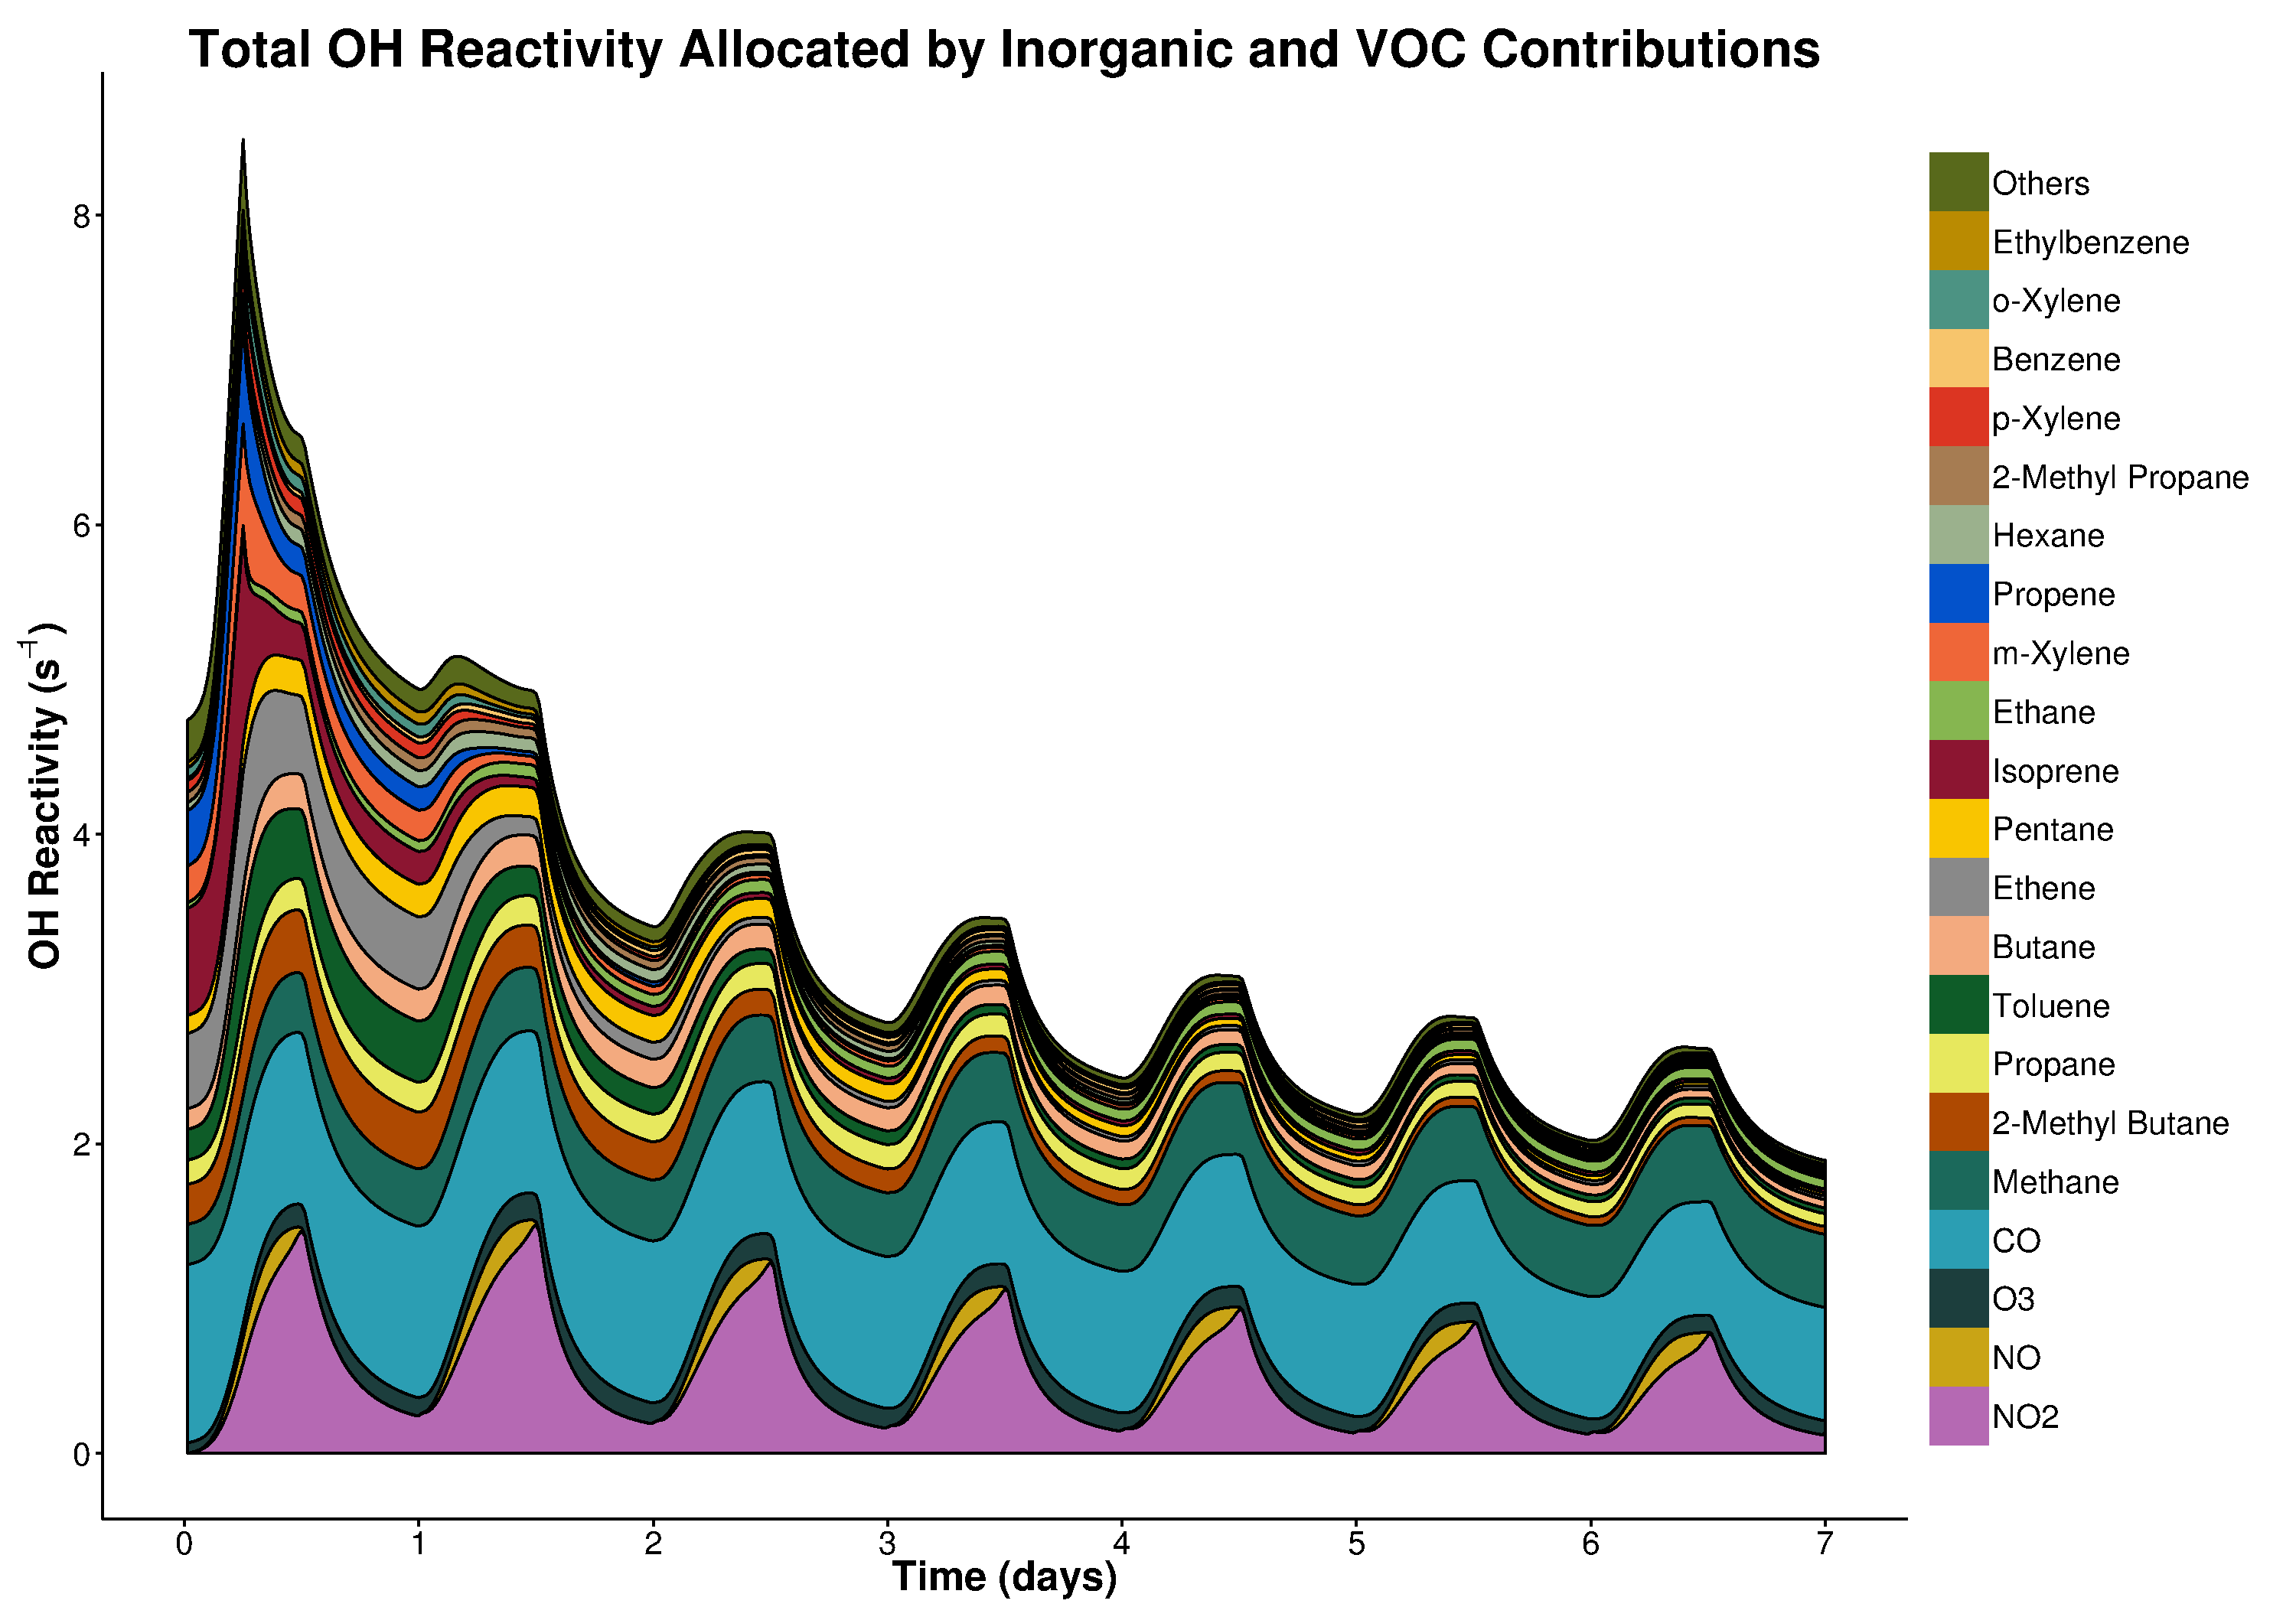
\includegraphics[scale=0.43]{img/OH_reactivity_allocation_time_series}
                \end{flushleft} 
                \column{.3\textwidth}
                    \begin{center} 
                        \textcolor{TitleBlue}{\textbf{\ce{O3} Reactivity}} 
                        \vskip3cm
                        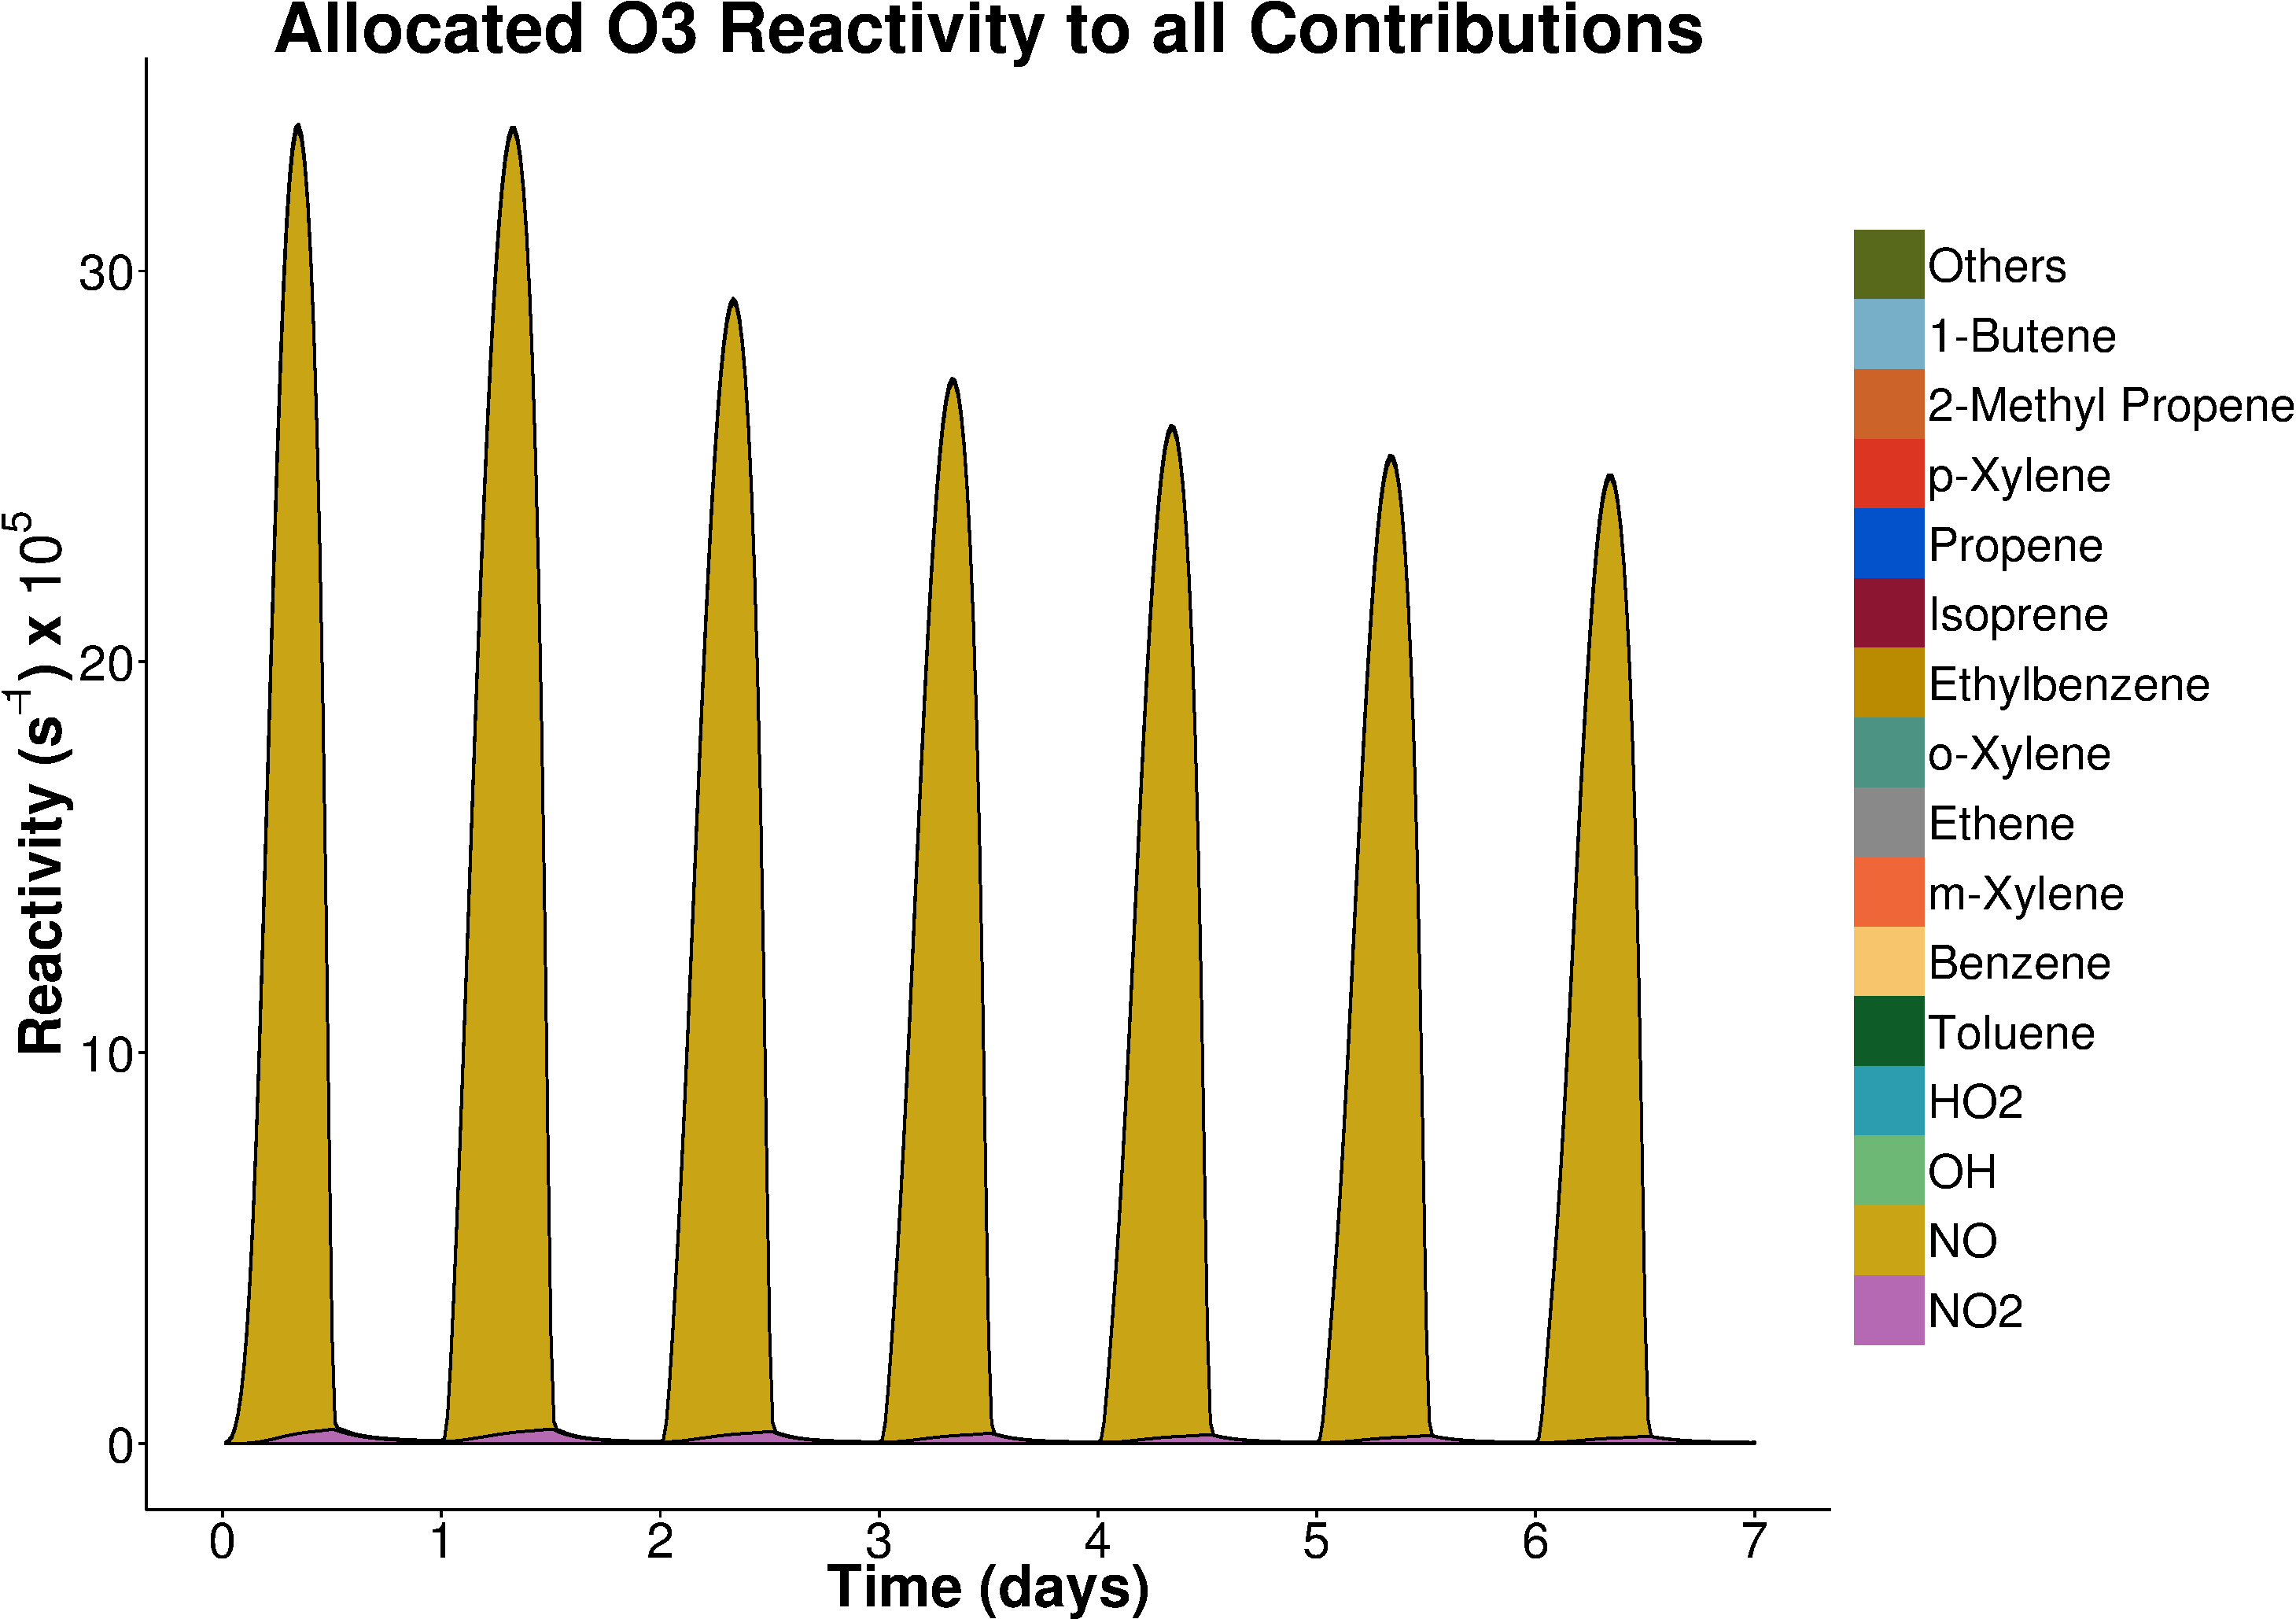
\includegraphics[scale=0.43]{img/O3_reactivity_allocation}
                        \vskip6cm
                        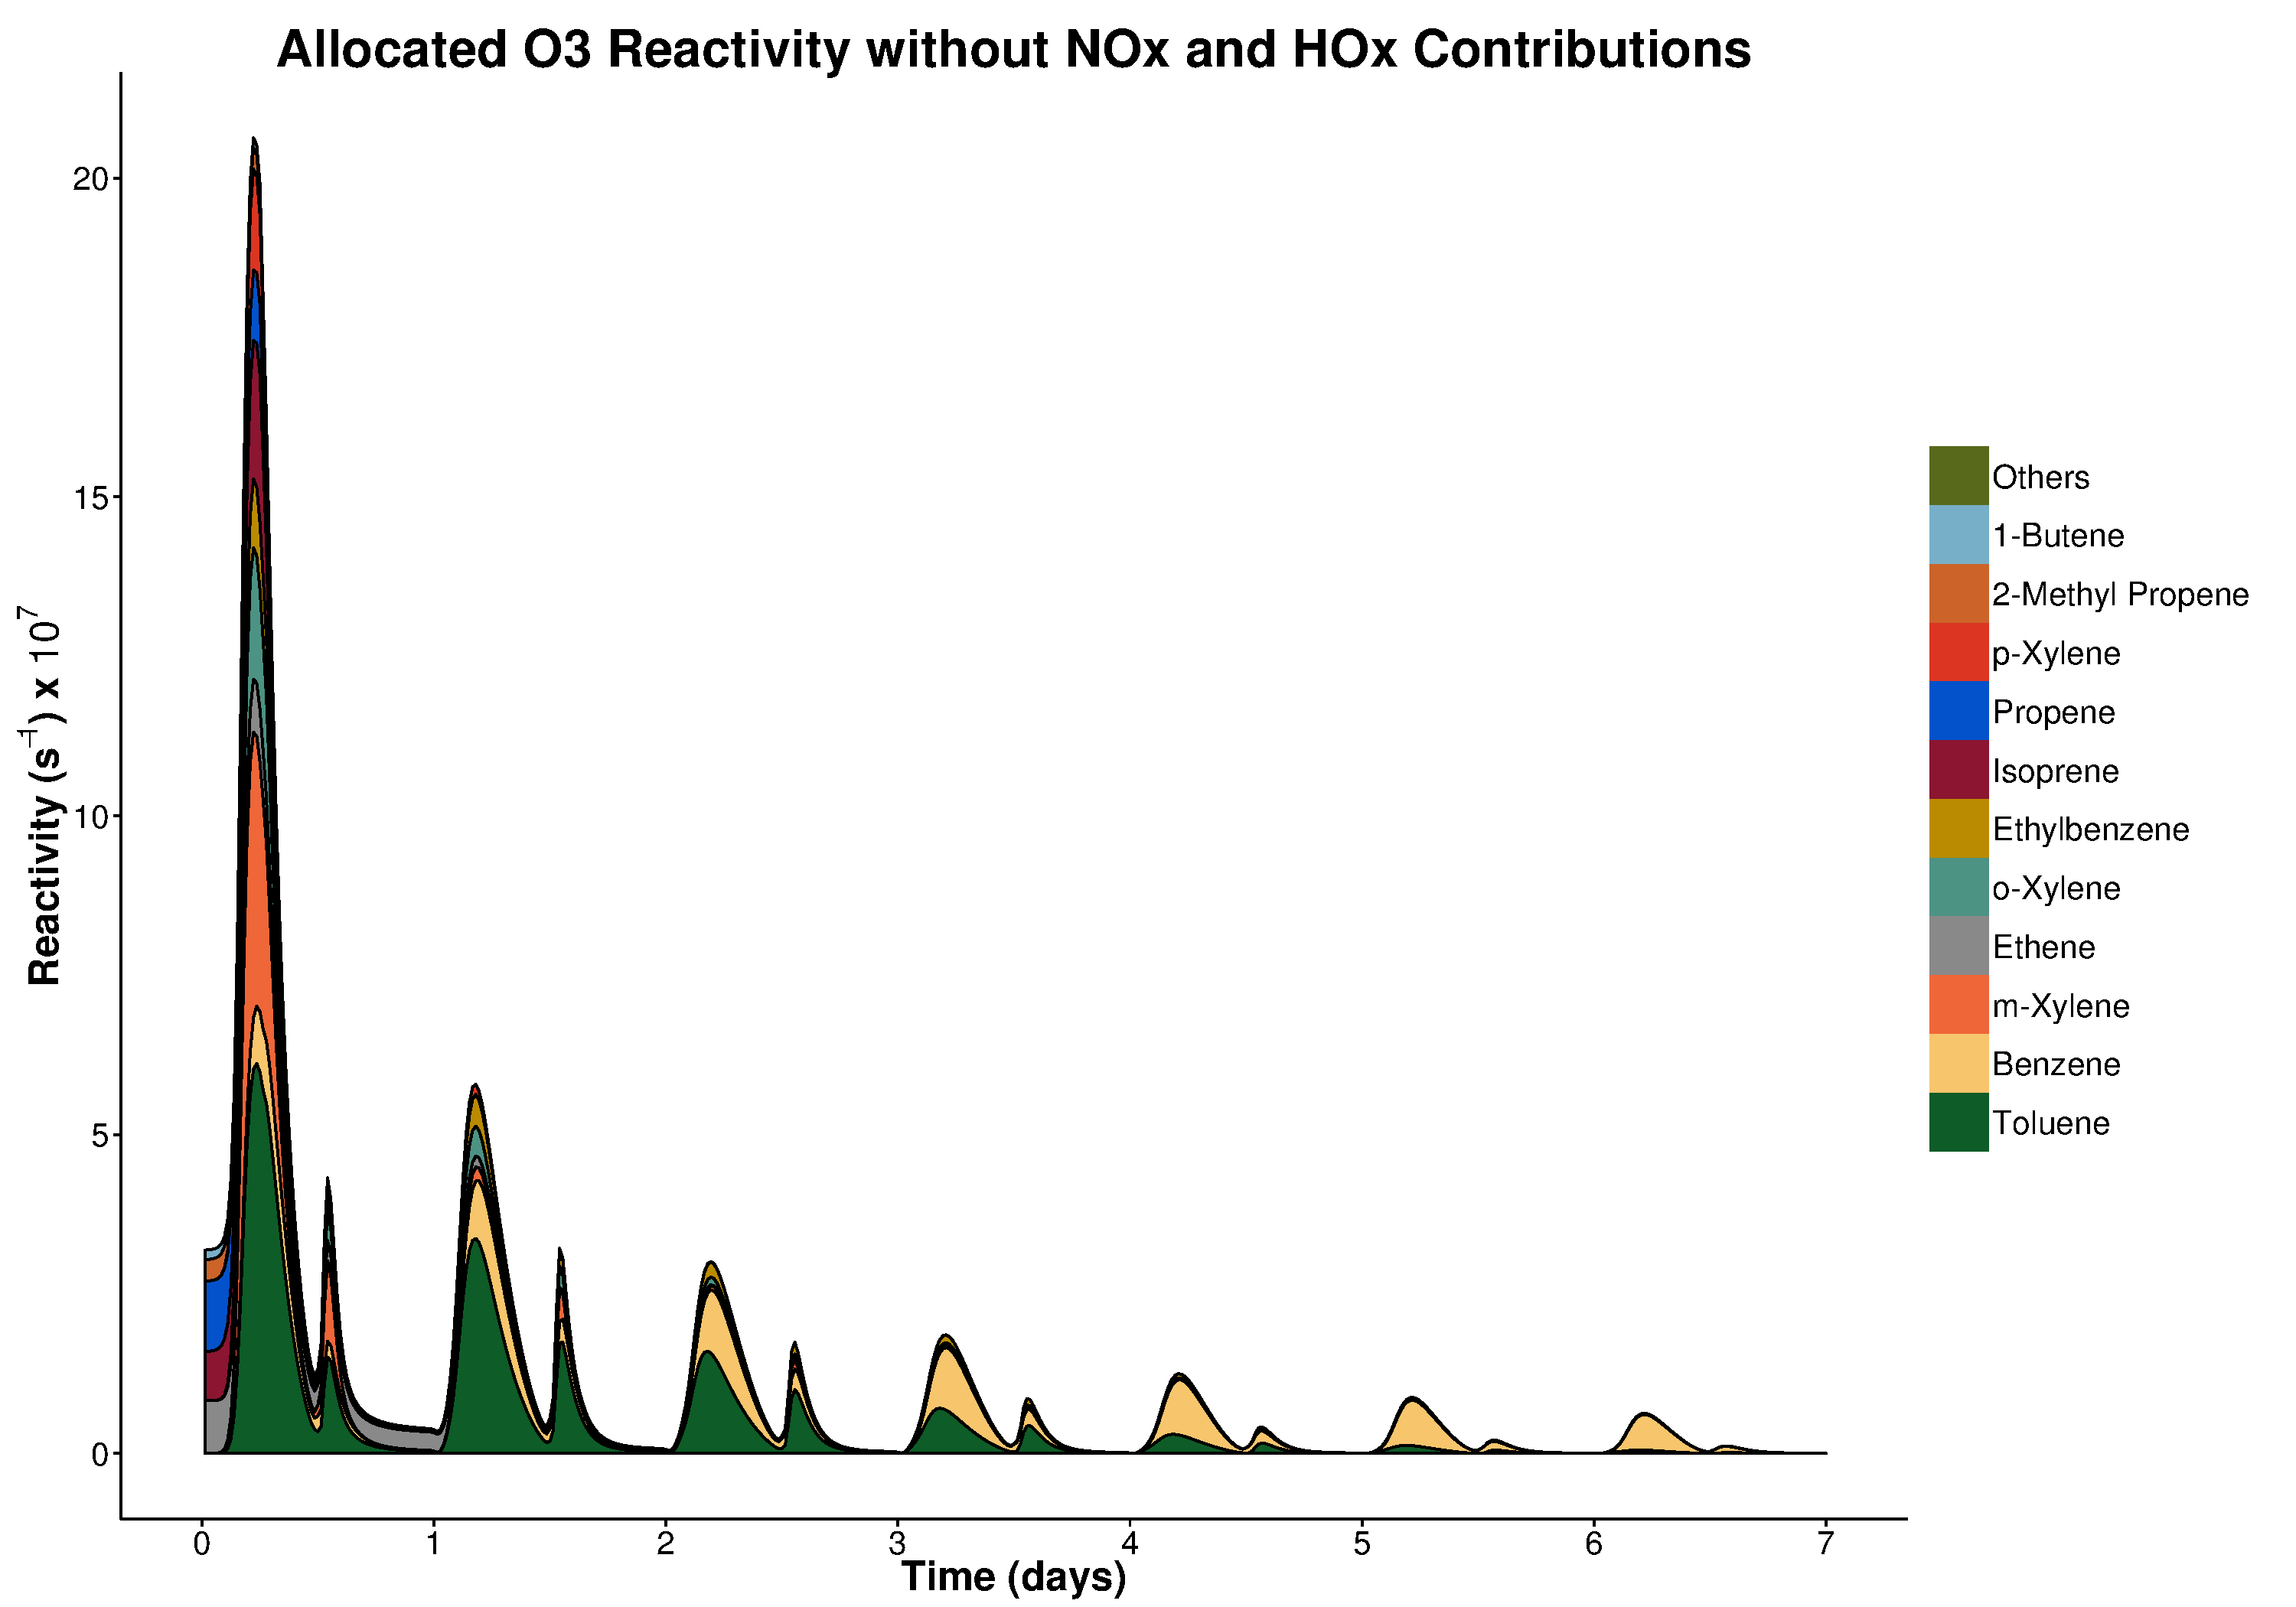
\includegraphics[scale=0.43]{img/O3_reactivity_allocation_without_NOx} 
                    \end{center}
                \column{.3\textwidth}
                    \begin{flushright}
                        \begin{center}\textcolor{TitleBlue}{\textbf{\ce{NO3} Reactivity}}\end{center}
                        \vskip3cm
                        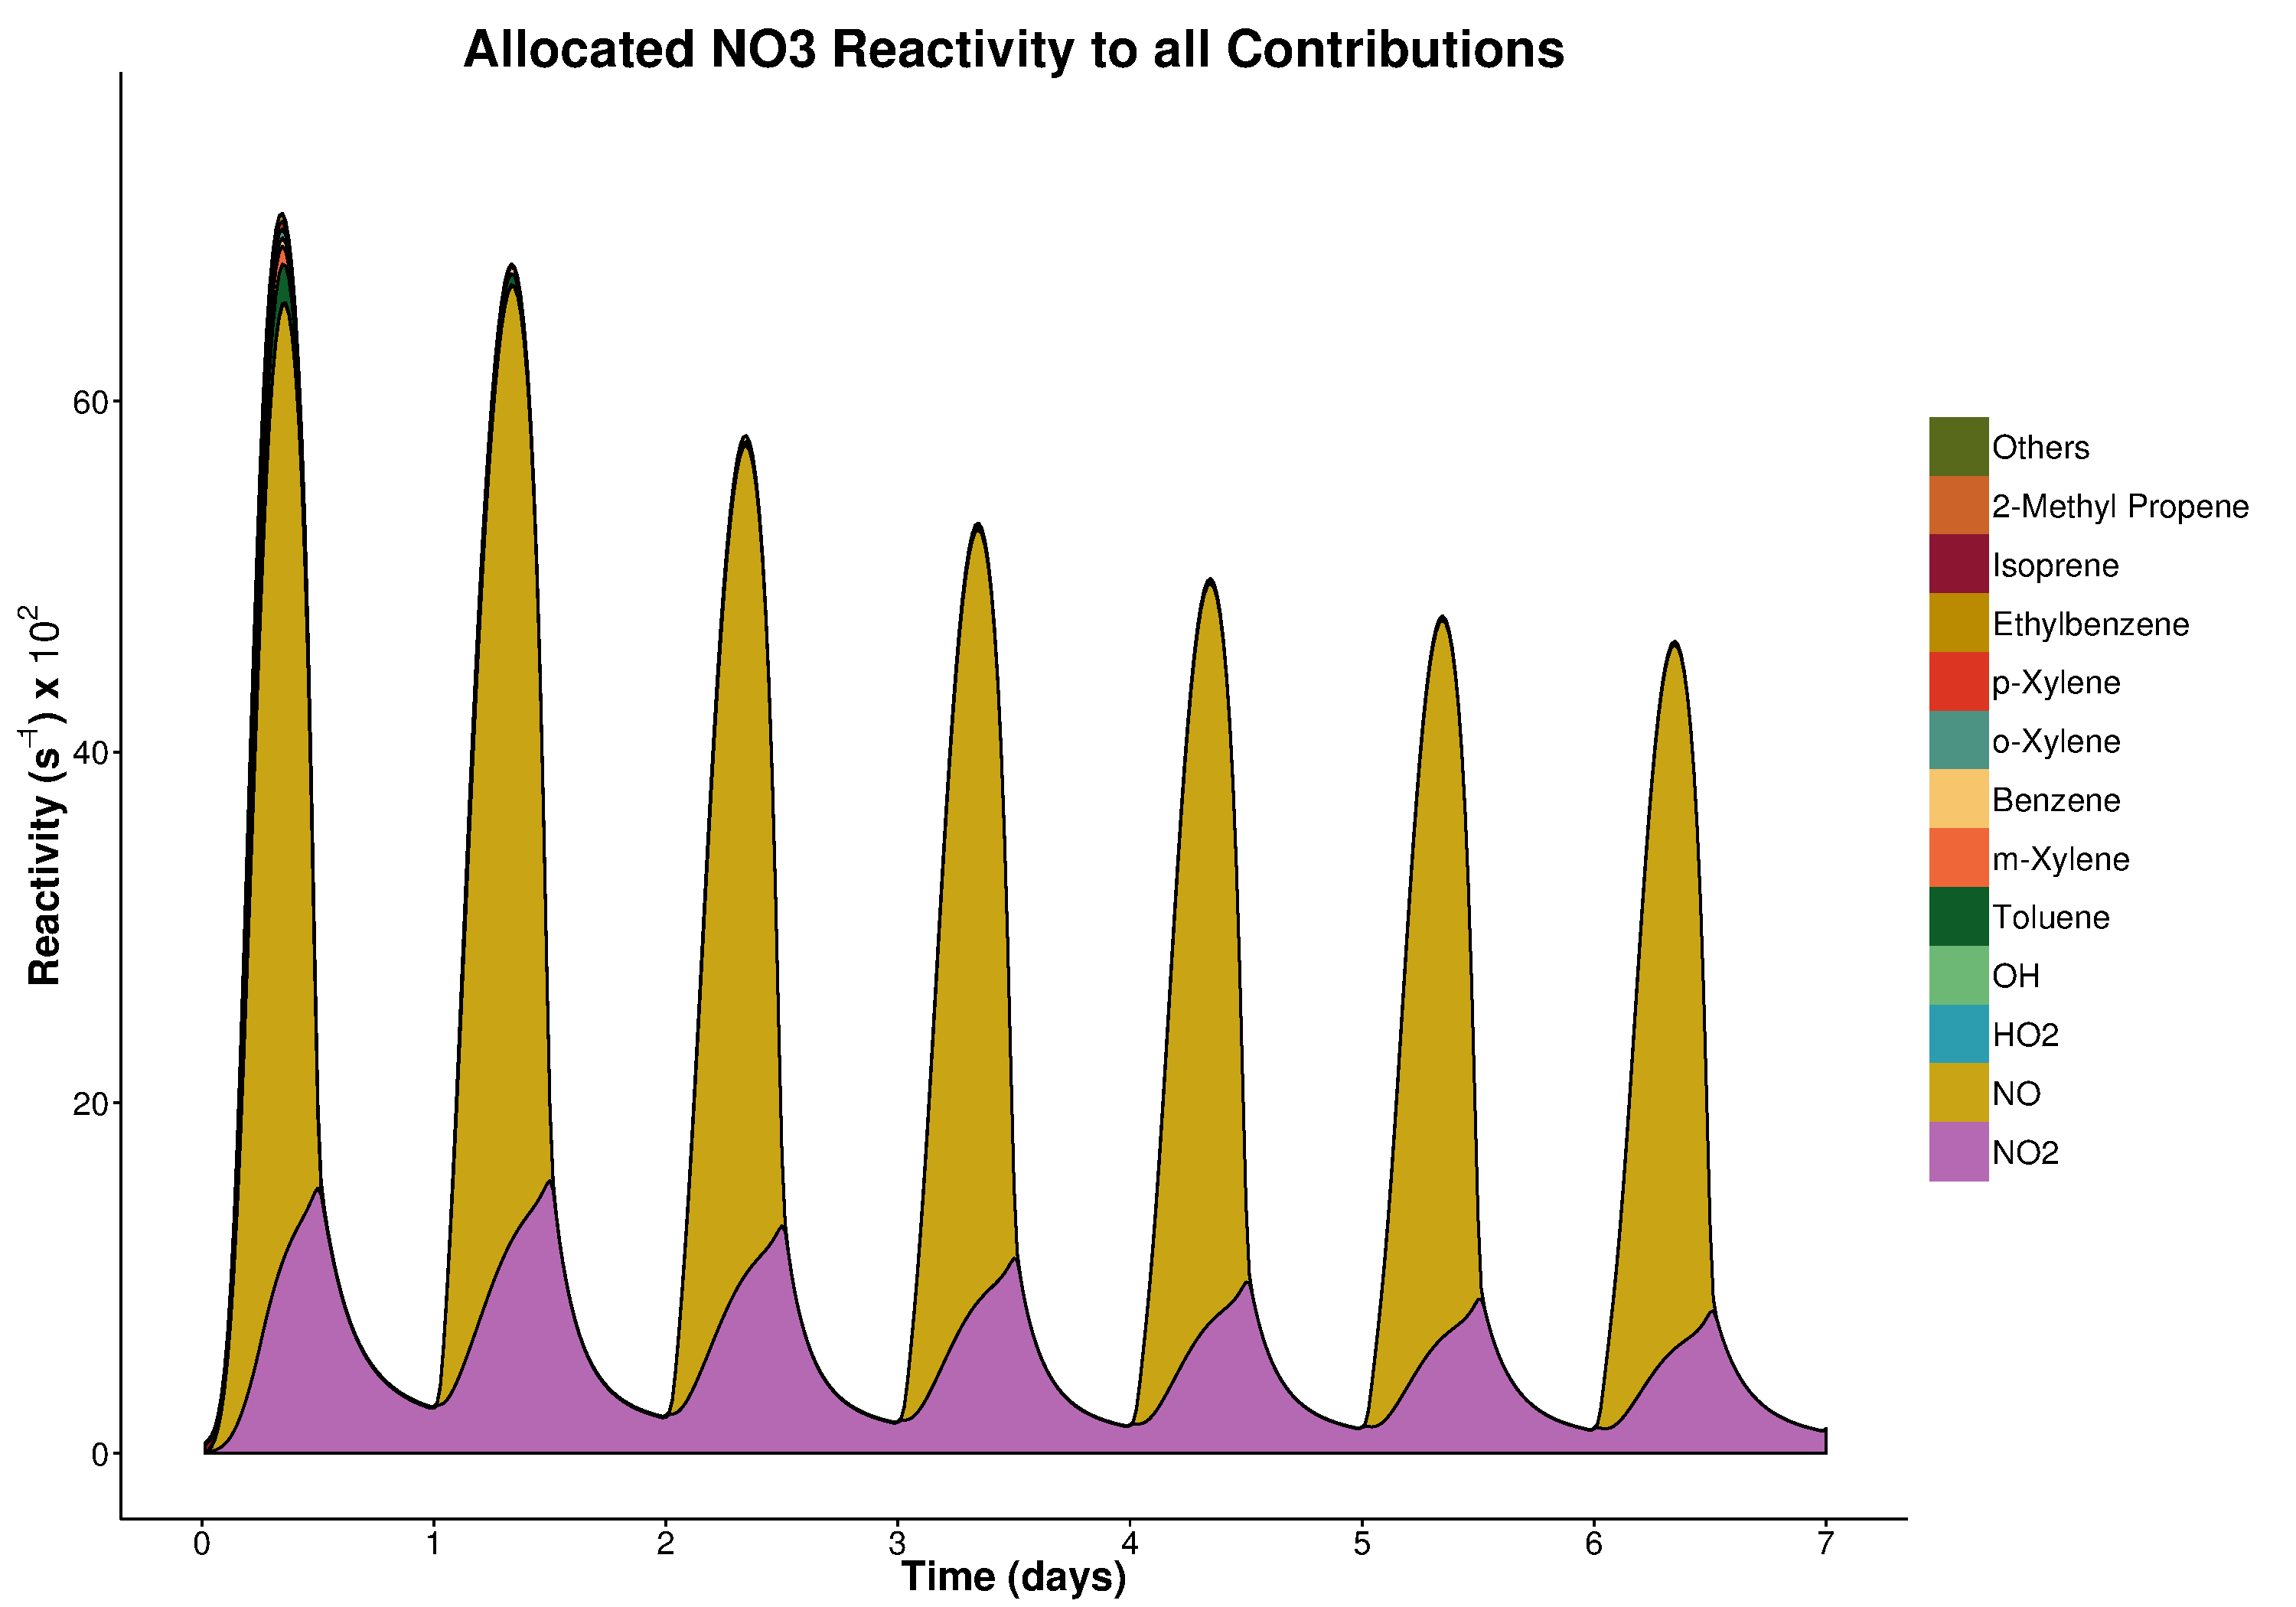
\includegraphics[scale=0.43]{img/NO3_reactivity_allocation}
                        \vskip6cm
                        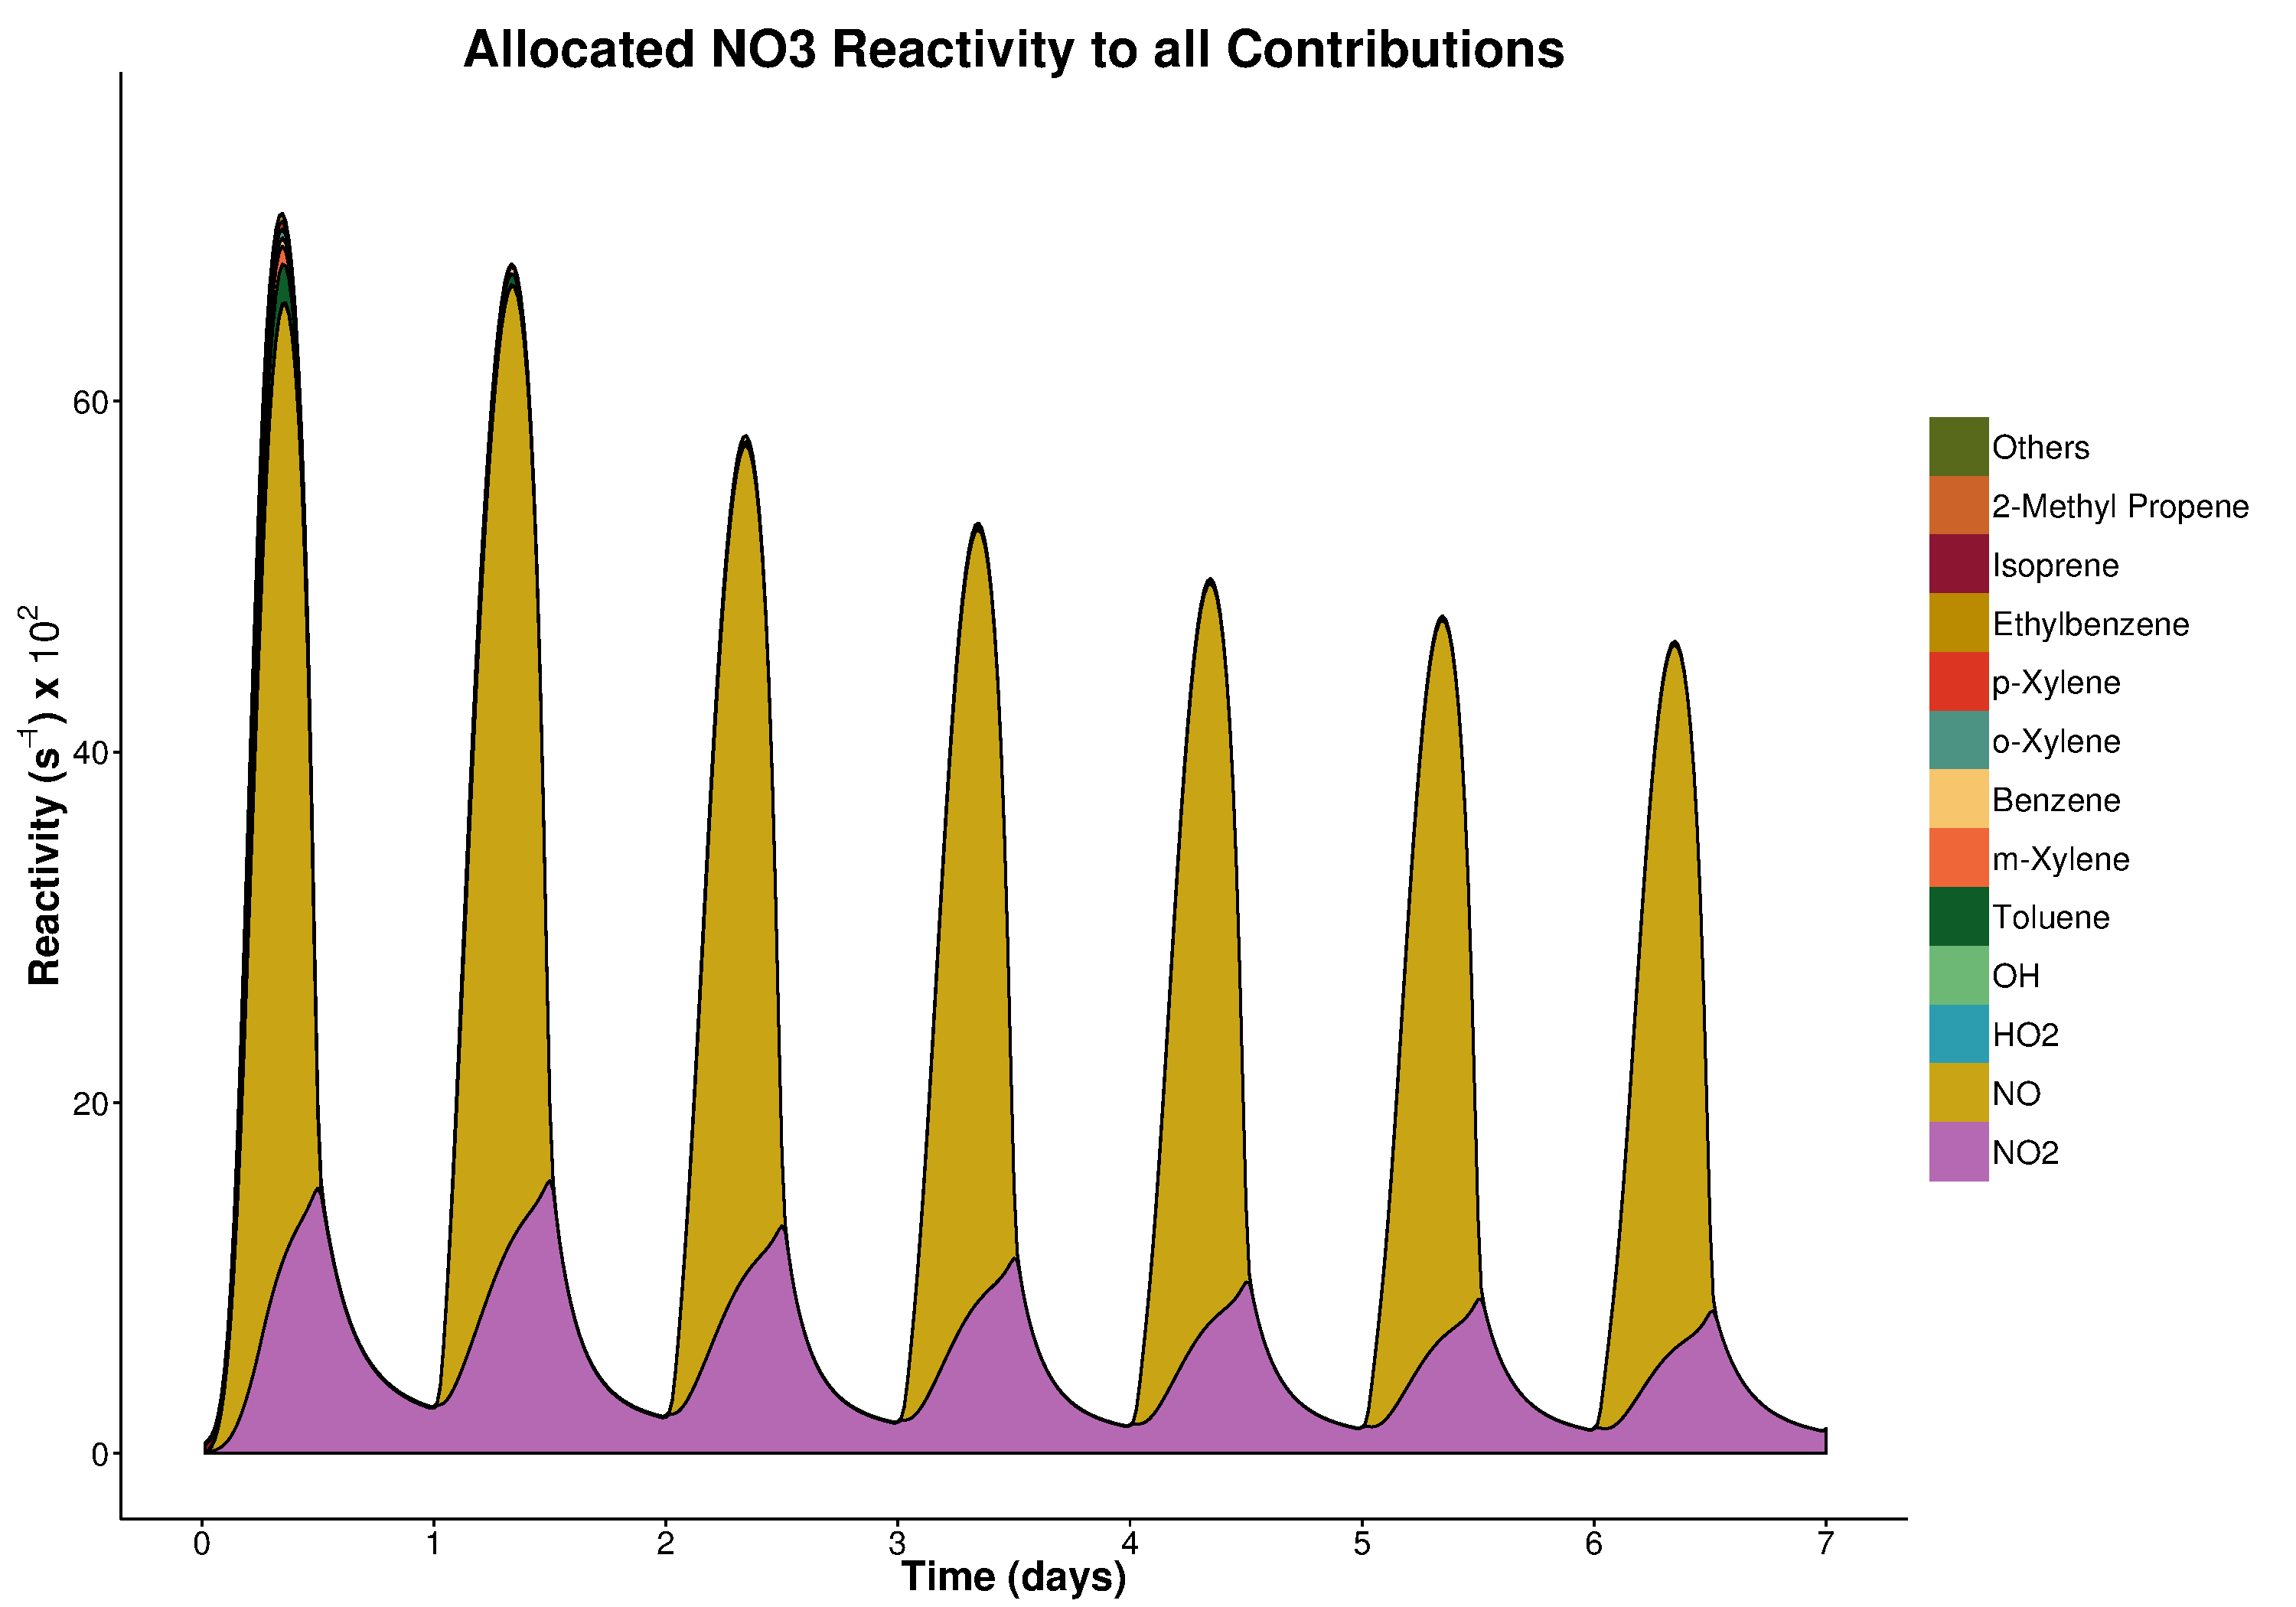
\includegraphics[scale=0.43]{img/NO3_reactivity_allocation_without_NOx}
                    \end{flushright}
        \end{columns}
        \begin{tikzpicture}[ultra thick, overlay]
            \node (placement) {};
            \node (dummy_OH_top) [above = 41cm of placement] {};
            \node (OH_top) [right = 23.5cm of dummy_OH_top] {};
            \node (OH_bottom) [right = 23.5cm of placement] {};
            \path [line width = 6mm, fill = TitleBlue, draw = TitleBlue] (OH_top) edge node {} (OH_bottom);

            \node (O3_top) [right = 48.5cm of dummy_OH_top] {};
            \node (O3_bottom) [right = 48.5cm of placement] {};
            \path [line width = 6mm, fill = TitleBlue, draw = TitleBlue] (O3_top) edge node {} (O3_bottom);
        \end{tikzpicture}
    \end{block}
\end{GreyBox}
